\documentclass[12pt]{article}
\usepackage{xcolor}
\usepackage{booktabs}
\usepackage{csquotes}
\usepackage{langsci-gb4e}
\usepackage{hyperref}
\hypersetup{
    colorlinks=true,
    linkcolor=blue,
    filecolor=magenta,
    citecolor=blue,      
    urlcolor=cyan,
    pdftitle={Grammaticality-deidealized},
    pdfpagemode=FullScreen,
}

\definecolor{lsDOIGray}{RGB}{0,0,0}
\usepackage[style=langsci-unified,backend=biber]{biblatex}
\addbibresource{refs.bib}
\usepackage{amsmath}
\usepackage{amssymb}
\usepackage{tcolorbox}
\usepackage{tikz}
\usepackage{microtype}
\usepackage{float}
\usepackage{orcidlink}
\usetikzlibrary{arrows.meta,shapes,positioning}

% Define only used colors
\definecolor{lsLightBlue}{RGB}{201,233,246}

\title{Grammaticality de-idealized: A community-based framework for understanding linguistic acceptability}
\author{Brett Reynolds \orcidlink{0000-0003-0073-7195}\\Humber Polytechnic \& University of Toronto
\thanks{I used ChatGPT o3-pro and Claude Opus 4 in drafting this version of the paper.\\This work is licensed under CC-BY 4.0}}
\date{\today}

\title{Grammaticality de-idealized\\[4pt]
       \large Lingbuzz preprint v0.3\\[6pt]
       \normalsize \url{https://github.com/BrettRey/Grammaticality-de-idealized-v2}}
\author{Brett Reynolds \orcidlink{0000-0003-0073-7195}\\Humber Polytechnic \& University of Toronto
\thanks{I used ChatGPT o1-preview and Claude Opus 4 in drafting this version of the paper.\\This work is licensed under CC-BY 4.0}}
\date{\today}

\begin{document}
\maketitle

\begin{abstract}
Speakers reject *\textit{I've finished it yesterday} yet accept the semantically odd \textit{Colorless green ideas sleep furiously}. They block *\textit{Which did you buy car?} categorically, while linguists judge the unreadable center-embedding \textit{The rat the cat the dog chased killed ate the cheese} as ``grammatical.'' This paper argues that such contrasts reflect grammaticality's true nature: the stability of community-specific morphosyntactic form–meaning pairings. Five interacting components determine an utterance's status: conventional morphosyntactic–meaning pairings, compatibility between those meanings and contextual meaning, incremental-processing limits, degree of community entrenchment, and categorical structural bans. This framework explains why processing overload can make grammatical sentences feel wrong, why compelling semantics can mask true violations, and which violations should improve under exposure. Grounding grammaticality in community conventions while acknowledging universal processing constraints, the approach unifies phenomena that elude purely formal or purely usage-based accounts.
\end{abstract}

\section{The puzzle of grammaticality}

Every competent speaker of English knows that *\textit{Can the have running} is impossible, but explaining this certainty proves remarkably difficult. Traditional approaches have struggled with three fundamental tensions. First, formal theories treat grammaticality as categorical, yet speakers consistently provide gradient judgments. \textcite{chomsky1965}'s competence-performance distinction attempted to resolve this by attributing gradience to processing limitations, but as \textcite[71]{schutze2016} notes, this allows supportive data to count as grammar while contrary data becomes ``performance noise.'' Consider center-embedded relatives like \textit{The bread the baker the apprentice helped made is delicious}, routinely labeled ``grammatical but unprocessable''—a description that merely restates rather than explains why speakers feel them to be wrong.

Second, the relationship between form and meaning in grammaticality remains contentious. While \textit{Colorless green ideas sleep furiously} demonstrates syntactic well-formedness without semantic plausibility, the converse also matters: speakers reject *\textit{I've finished it yesterday} because the present perfect's current relevance meaning clashes with the adverb's completed past specification. Construction grammar \parencite{goldberg1995constructions} confirms that morphosyntactic and lexical meanings must cohere, explaining why \textit{She texted him the address} succeeds while *\textit{She disappeared him the evidence} fails.

Third, universal principles conflict with community conventions. \textcite{labov1972} demonstrated that grammaticality is community-relative, with languages differing not just lexically but in which form–meaning pairings become conventionalized. Usage-based models capture frequency effects but still face cases where extremely rare patterns remain grammatical while frequent patterns are blocked.

This paper proposes that these tensions dissolve when we recognize grammaticality as the community stability of morphosyntactic form–meaning pairings. Rather than an autonomous syntactic property or simple frequency effect, grammaticality emerges from the interaction of five components: morphosyntactic pairings, contextual meaning compatibility, processing constraints, community entrenchment, and structural bans. This framework explains gradient judgments, form-meaning interactions, and cross-linguistic variation while making testable predictions about language change and acquisition.

\section{Five components of grammaticality}

Grammaticality emerges when morphosyntactic forms establish stable, conventional pairings with meanings within specific language communities. This stability depends on five interacting components, each contributing to whether an utterance achieves grammatical status.

The first component requires viable morphosyntactic form–meaning pairings within the relevant community. Some utterances simply fail to map form onto any recognizable meaning pattern. Consider *\textit{Can the have running?}, where the modal \textit{can} expects a subject and verb phrase to form a coherent proposition, but \textit{the have running} yields neither a legitimate noun phrase nor verbal structure. With no stable pairing to anchor interpretation, the utterance remains nonsensical. In contrast, \textit{Colorless green ideas sleep furiously} succeeds here because despite semantic oddity, it presents a clear compositional morphosyntactic structure pairing with compositional meaning.

Community conventions shape which pairings are recognized as legitimate. Spanish-English bilingual speakers may accept \textit{Estábamos lifting en el gym} (`We were lifting in the gym'), where Spanish progressive morphology combines with English vocabulary in a pattern conventional within that bilingual community but ungrammatical in monolingual contexts. This demonstrates how grammaticality depends not on universal principles but on community-specific conventions about acceptable form–meaning combinations.

The second component demands compatibility between morphosyntactic meanings and contextual meanings drawn from lexical semantics, discourse context, and pragmatic inference. Even well-formed morphosyntactic structures become ungrammatical when they clash with contextual meanings. The rejection of *\textit{I've finished it yesterday} illustrates this: the present perfect construction encodes current relevance while \textit{yesterday} specifies completed past time, creating an irreconcilable temporal contradiction. Similarly, *\textit{I have 25 years} fails in English age expressions because \textit{have} + \textit{years} conventionally denotes temporal duration or possession rather than age attribution.

Information-structural conflicts also trigger this type of ungrammaticality. In *\textit{Who did the lifeguard who saved \_ work in New Jersey?}, the same participant is simultaneously focused through \textit{wh}-movement while being backgrounded in the relative clause, creating incompatible information-structural requirements \parencite{CuneoGoldberg2023}. Such semantic incompatibilities make constructions ungrammatical even when individual morphosyntactic components are properly formed.

The third component involves processing constraints that emerge from memory limitations and incremental parsing demands. When constructions exceed cognitive capacity, they trigger ungrammaticality feelings despite structural well-formedness. Multiple center embeddings exemplify this pattern, where incremental processing becomes impossible as in \textit{The rat the cat the dog chased killed ate the cheese}. Evidence from parsing studies \parencite{gibson2000} shows that dependencies spanning multiple intervening elements increase processing difficulty, with new referents between dependent elements compounding memory load.

Rather than reflecting simple memory limitations, processing constraints emerge from interactions between specialized language networks and domain-general cognitive systems \parencite{Fedorenko2024}. The parallel evolution of these neural networks suggests that processing difficulty reflects optimization pressures for efficient communication across brain systems rather than a single cognitive bottleneck. This architecture explains why simpler, more memorable forms tend to spread through languages over time, as speakers preferentially select structures that minimize cross-network processing demands.

The fourth component captures community entrenchment—the degree to which form–meaning pairings have become conventionalized within a speech community. Even transparent, processable constructions fail when they violate established conventions. Regular plural *\textit{sheeps} demonstrates this: the morphosyntactic pattern is semantically transparent and structurally parallel to other English plurals, yet speakers reject it because the community has entrenched the irregular form \textit{sheep}. Without metaphorical or playful justification, the regularized version remains unacceptable.

Community entrenchment operates independently from other components. Constructions may achieve perfect semantic compatibility and minimal processing demands yet still face rejection because communities have conventionalized different forms for those meanings. The independent relative \textit{whose}, as in \textit{I saw Joan, a friend of whose was visiting}, illustrates this pattern. While analogically related to accepted constructions, its extreme rarity prevents stable conventionalization, leaving speakers uncertain about its status despite its potential grammaticality.

The fifth component involves categorical structural constraints that resist explanation through the other factors. Some constructions face systematic blocking independent of meaning, processing, or community acceptance. Left-branch extraction (*\textit{Which did you buy \_ car?}) exemplifies this pattern. The intended meaning `Which car did you buy?' is transparent and the construction poses no unusual processing demands, yet English categorically prohibits extracting determiners alone from noun phrases. As \textcite{Snyder2022} note, no study has found reliable satiation effects for such violations, suggesting truly categorical blocking.

These categorical constraints represent extreme stability biases rather than inviolable universal principles. While cross-linguistically robust, they emerge from community-specific historical processes rather than innate constraints. The framework treats them as community entrenchment extremes where acceptability approaches zero, though future work might test their potential malleability under unusual sociolinguistic conditions.

\section{A diagnostic framework}

These five components can be organized into a decision tree that provides first-pass classification of utterances. The tree identifies the first component whose failure renders an utterance ungrammatical, with later factors evaluated only when earlier ones succeed.

\begin{figure}[H]
\centering
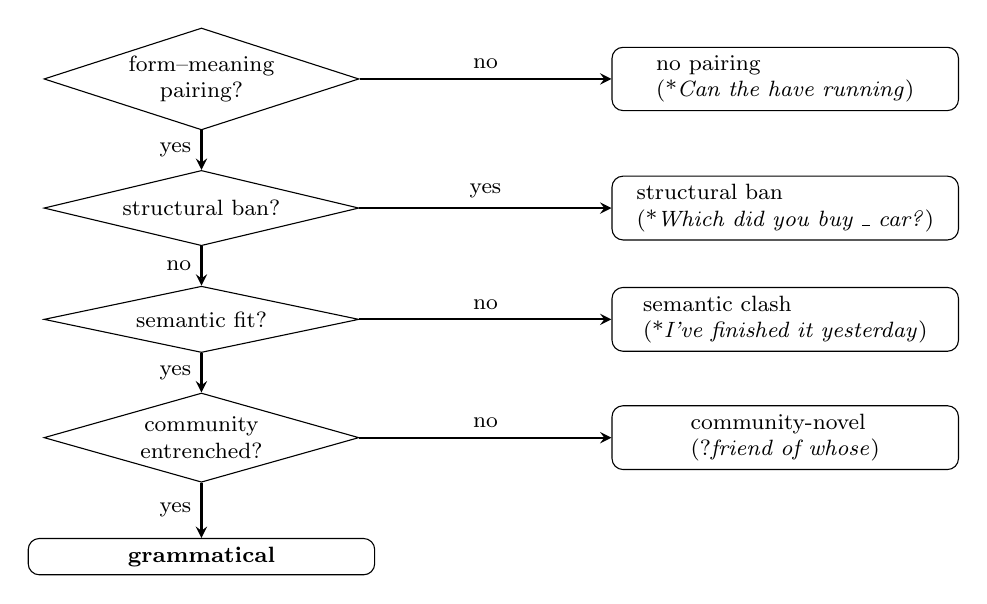
\begin{tikzpicture}[
  font=\footnotesize,                       % smaller text everywhere
  node distance = 0.5cm and 3.2cm,         % tighter vertical gap
  decision/.style = {diamond,
                     aspect=3,              % width : height = 3 : 1  →  flatter
                     draw,
                     align=center,
                     minimum width=4cm,
                     inner sep=1pt},
  outcome/.style  = {rectangle,
                     draw,
                     rounded corners,
                     align=left,
                     minimum width=4.4cm,
                     inner sep=3pt},
  arrow/.style    = {->, >=stealth, thick}
]

\node[decision] (map)  {form–meaning\\pairing?};
\node[outcome , right=of map]  (nonsense) {no pairing\\(*\textit{Can the have running})};

\node[decision, below=of map]  (ban)  {structural ban?};
\node[outcome , right=of ban]  (lbe)  {structural ban\\(*\textit{Which did you buy \_ car?})};

\node[decision, below=of ban]  (sem)  {semantic fit?};
\node[outcome , right=of sem]  (clash) {semantic clash\\(*\textit{I've finished it yesterday})};

\node[decision, below=of sem]  (ent)  {community\\entrenched?};
\node[outcome , right=of ent]  (novel) {community‑novel\\(?\textit{friend of whose})};

\node[outcome , below=0.7cm of ent] (gram) {\textbf{grammatical}};

\draw[arrow] (map)  -- node[above] {no} (nonsense);
\draw[arrow] (map)  -- node[left]  {yes} (ban);
\draw[arrow] (ban)  -- node[above] {yes} (lbe);
\draw[arrow] (ban)  -- node[left]  {no}  (sem);
\draw[arrow] (sem)  -- node[above] {no}  (clash);
\draw[arrow] (sem)  -- node[left]  {yes} (ent);
\draw[arrow] (ent)  -- node[above] {no}  (novel);
\draw[arrow] (ent)  -- node[left]  {yes} (gram);

\end{tikzpicture}
\caption{Decision tree for first‑pass diagnosis.}
\end{figure}


This heuristic diagnostic tool helps distinguish different sources of ungrammaticality that traditional approaches often conflate. Form-meaning mapping failures like *\textit{Can the have running} differ qualitatively from semantic clashes like *\textit{I've finished it yesterday}. Each type of violation reflects different underlying causes and should show different behavioural signatures in experimental settings.

\begin{tcolorbox}[colback=lsLightBlue!15]
\textbf{Note.} The tree classifies utterances on the dimension of
\emph{objective grammaticality}. A sentence can pass the tree but yield a \emph{feeling} of ungrammaticality if either the diagnostic weight or processing cost is high (see Section \ref{sec:obj-subj}).
\end{tcolorbox}

\section{Objective grammaticality versus subjective feelings}\label{sec:obj-subj}

\begin{figure}[htbp]
\centering
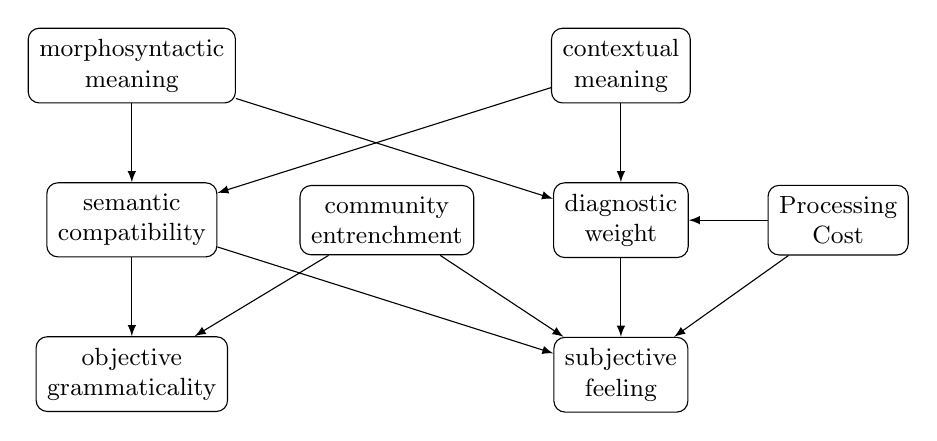
\begin{tikzpicture}[
  node distance = 1cm and 4.0cm,
  > = latex,
  var/.style = {rectangle, draw, rounded corners, align=center,
                inner sep=4pt, font=\small}
]

\node[var] (mu)    {morphosyntactic\\meaning};
\node[var, right=of mu] (sigman) {contextual\\meaning};

\node[var, below=of mu]     (K) {semantic\\compatibility};
\node[var, below=of sigman]  (r) {diagnostic\\weight};

\node[var, left=1cm of r] (C) {community\\entrenchment};

\node[var, below=of K]      (G) {objective\\grammaticality};
\node[var, below=of r]      (F) {subjective\\feeling};

\node[var, right=1cm of r] (P) {Processing\\Cost};

\draw[->] (mu)    -- (K);
\draw[->] (sigman) -- (K);
\draw[->] (mu)    -- (r);
\draw[->] (sigman) -- (r);
\draw[->] (K) -- (G);
\draw[->] (C) -- (G);
\draw[->] (K) -- (F);
\draw[->] (r) -- (F);
\draw[->] (C) -- (F);
\draw[->] (P) -- (r);
\draw[->] (P) -- (F);
\end{tikzpicture}
\caption{Causal structure of grammaticality judgments}\label{fig:causal-dag}
\end{figure}

A crucial insight emerges from distinguishing objective grammaticality—whether a form–meaning pairing is licensed within a community—from subjective feelings of ungrammaticality that speakers experience. This distinction parallels other metacognitive phenomena like the feeling of knowing, where we sense certainty about information we cannot retrieve \parencite{hart1965}.

Objective grammaticality depends on the stability of community-recognized form–meaning pairings, while subjective feelings reflect speakers' metacognitive responses to perceived violations. These can diverge systematically. Grammatical constructions may feel ungrammatical when processing demands overwhelm cognitive resources, as with center embeddings. Conversely, ungrammatical constructions may escape detection when semantic content provides compelling interpretations, masking underlying structural violations.

Consider \textit{The old man the boats}, which initially feels ungrammatical due to garden-path effects \parencite{ritchie1984}. Readers typically parse \textit{old man} as a noun phrase, yielding nonsense. But the sentence is actually grammatical with \textit{the old} as subject (meaning `elderly people') and \textit{man} as verb (`operate'). The feeling of ungrammaticality reflects processing difficulty rather than structural violation.

Agreement errors demonstrate the opposite pattern: *\textit{The patchwork of laws governing background checks help explain why people continue to be wounded} contains a genuine violation where singular \textit{patchwork} clashes with plural \textit{help}, but intervening plural nouns mask this error \parencite{corbett2016}. Cognitive resources devoted to processing complexity prevent detection of the actual violation.

The causal structure underlying grammaticality judgments can be represented as a directed acyclic graph (Figure \ref{fig:causal-dag}) showing how different factors contribute to both objective grammaticality and subjective feelings.



This model shows how morphosyntactic meaning and contextual meaning combine to determine semantic compatibility, which affects both objective grammaticality (through community entrenchment) and subjective feelings (through detectability and processing costs). The framework predicts that experimental manipulations of familiarity or processing load will shift subjective feelings without necessarily changing objective grammatical status.

\section{Implications for grammatical theory}

This framework reconciles insights from multiple theoretical traditions while making novel predictions about grammatical phenomena. Unlike purely formal approaches, it explains why meaning matters for grammaticality judgments. Unlike purely usage-based approaches, it accounts for systematic gaps where frequent patterns are blocked and rare patterns remain grammatical. Unlike processing-only accounts, it explains categorical constraints that resist amelioration through exposure.

The approach yields specific testable predictions. First, satiation effects—where repeated exposure increases acceptability—should occur for constructions where ungrammaticality stems from low frequency, processing difficulty, or weak morphosyntactic integration, but not for categorical structural violations. Second, cross-linguistic variation in grammaticality judgments should correlate with differences in how tightly morphosyntactic and lexical meanings are integrated. Languages like Spanish, where grammatical gender permeates morphosyntax, should show stronger ungrammaticality for gender mismatches than English, where gender integration is weaker. Third, second-language learners should initially perceive unfamiliar input as meaningless noise rather than explicitly ungrammatical, then show heightened sensitivity to violations before gradually aligning with native-speaker norms.

The framework also illuminates grammatical change by identifying when innovations become entrenched. Constructions gain acceptance when community dynamics favor them over alternatives, driven by semantic transparency, social prestige, structural analogy, or iconic relationships between form and meaning. The logistic growth patterns observed in language change emerge naturally from these community-level dynamics.

\section{Community dynamics and language change}

Understanding grammaticality as community-based form–meaning stability explains both synchronic variation and diachronic change. Different communities conventionalize different pairings based on their communicative needs, social structures, and historical trajectories. What counts as grammatical thus varies across dialects, registers, and social groups, not because grammar is arbitrary but because different communities establish different stable solutions to similar communicative problems.

Multiple modal constructions illustrate this community relativity. Some American English speakers systematically accept \textit{I might could help you with that}, productively generating similar combinations \parencite{morin2024semantics}. Speakers from single-modal communities typically reject such combinations as ungrammatical. This variation reflects different community conventions about acceptable modal combinations rather than differences in underlying competence.

Change occurs when community dynamics shift to favor innovations over established patterns. This happens through various mechanisms: semantic reanalysis that makes form–meaning relationships more transparent, social motivations that associate forms with desired group identities, structural pressures from analogy or processing constraints, or iconic relationships that make form–meaning connections more natural. The development of \textit{going to} future illustrates semantic reanalysis, where directional motion toward goals was reinterpreted as temporal movement toward future events.

The framework predicts that successful innovations will show S-curve adoption patterns as they spread through communities. Initial slow growth reflects resistance from established conventions, followed by rapid acceleration once social tipping points are reached, then deceleration as the innovation approaches community-wide acceptance. This pattern emerges naturally from the interaction between individual adoption decisions and community-level feedback effects.

\section{Conclusion}

Grammaticality emerges from the stability of morphosyntactic form–meaning pairings within language communities, modulated by processing constraints and social factors. This framework unifies categorical and gradient phenomena, explains form-meaning interactions, and accounts for cross-linguistic variation while making testable predictions about satiation effects, language change, and acquisition patterns.

The approach moves beyond traditional competence-performance dichotomies by treating grammaticality as an emergent property of community practice rather than an autonomous formal system. Processing constraints, semantic compatibility, and social factors all contribute to which form–meaning pairings become stable, but none alone determines grammatical status. This interaction explains why some rare constructions remain grammatical while frequent patterns can be blocked, why processing difficulty can make grammatical sentences feel wrong, and why compelling semantics can mask structural violations.

Future research should test the framework's specific predictions about satiation effects, cross-linguistic variation, and acquisition trajectories. Corpus studies can track the community dynamics proposed to underlie grammatical change, while experimental work can distinguish objective grammatical status from subjective processing effects. Cross-linguistic investigation of how different degrees of morphosyntactic integration affect grammaticality judgments will be particularly valuable for validating the framework's core claims.

By grounding grammaticality in community conventions while acknowledging universal processing constraints, this approach provides a foundation for understanding how human communities create and maintain the systematic form–meaning relationships we call grammar. Rather than reducing grammaticality to formal rules, frequency effects, or processing limitations alone, it reveals how these factors interact to produce the rich patterns of acceptability that characterize human language.

\newpage
\begin{sloppypar}
\printbibliography[title=References]
\end{sloppypar}

\end{document}